%%%%%%%%%%%%%%%%%%%%%%%%%%%%%%%%%%%%%%%%%
% Daily Laboratory Book
% LaTeX Template
% Version 1.0 (4/4/12)
%
% This template has been downloaded from:
% http://www.LaTeXTemplates.com
%
% Original author:
% Frank Kuster (http://www.ctan.org/tex-archive/macros/latex/contrib/labbook/)
%
% Important note:
% This template requires the labbook.cls file to be in the same directory as the
% .tex file. The labbook.cls file provides the necessary structure to create the
% lab book.
%
% The \lipsum[#] commands throughout this template generate dummy text
% to fill the template out. These commands should all be removed when 
% writing lab book content.
%
% HOW TO USE THIS TEMPLATE 
% Each day in the lab consists of three main things:
%
% 1. LABDAY: The first thing to put is the \labday{} command with a date in 
% curly brackets, this will make a new page and put the date in big letters 
% at the top.
%
% 2. EXPERIMENT: Next you need to specify what experiment(s) you are 
% working on with an \experiment{} command with the experiment shorthand 
% in the curly brackets. The experiment shorthand is defined in the 
% 'DEFINITION OF EXPERIMENTS' section below, this means you can 
% say \experiment{pcr} and the actual text written to the PDF will be what 
% you set the 'pcr' experiment to be. If the experiment is a one off, you can 
% just write it in the bracket without creating a shorthand. Note: if you don't 
% want to have an experiment, just leave this out and it won't be printed.
%
% 3. CONTENT: Following the experiment is the content, i.e. what progress 
% you made on the experiment that day.
%
%%%%%%%%%%%%%%%%%%%%%%%%%%%%%%%%%%%%%%%%%

%----------------------------------------------------------------------------------------
%	PACKAGES AND OTHER DOCUMENT CONFIGURATIONS
%----------------------------------------------------------------------------------------

\documentclass[idxtotoc,hyperref,openany,oneside]{files/forensics} % 'openany' here removes the gap page between days, erase it to restore this gap; 'oneside' can also be added to remove the shift that odd pages have to the right for easier reading

\usepackage[ 
  backref=page,
  pdfpagelabels=true,
  plainpages=false,
  colorlinks=true,
  bookmarks=true,
  pdfview=FitB]{hyperref} % Required for the hyperlinks within the PDF
  
\usepackage{booktabs} % Required for the top and bottom rules in the table
\usepackage{float} % Required for specifying the exact location of a figure or table
\usepackage{graphicx} % Required for including images2
\usepackage{listings} % Used for programs' listings
\usepackage{tcolorbox} % For textboxes
\usepackage{hyperref}

\usepackage[english,russian]{babel}
\usepackage[utf8]{inputenc}
\usepackage[T2A]{fontenc}

\newcommand{\HRule}{\rule{\linewidth}{0.5mm}} % Command to make the lines in the title page
\setlength\parindent{0pt} % Removes all indentation from paragraphs

%----------------------------------------------------------------------------------------
%	DEFINITION OF EXPERIMENTS
%----------------------------------------------------------------------------------------

\newexperiment{easy1}{Baby keyboard}
\newexperiment{easy2}{Just log in}
\newexperiment{medium1}{Find file}
\newexperiment{medium2}{Do you hear it?}
\newexperiment{hard}{Random xor}
\newexperiment{reallife}{How about history?}

%---------------------------------------------------------------------------------------

\begin{document}

%----------------------------------------------------------------------------------------
%	TITLE PAGE
%----------------------------------------------------------------------------------------

\frontmatter % Use Roman numerals for page numbers
\title{
\begin{center}
\HRule \\[0.4cm]
{\Huge \bfseries CTF Code \\[0.5cm] \Large Writeups}\\[0.4cm] % Degree
\HRule \\[1.5cm]
\end{center}
}
\author{\Huge Forensics \\ \\[2cm]} % Your name and email address
\maketitle

\tableofcontents

\mainmatter % Use Arabic numerals for page numbers

%----------------------------------------------------------------------------------------
%	LAB BOOK CONTENTS
%----------------------------------------------------------------------------------------

% Blank template to use for new days:

%\labday{Day, Date Month Year}

%\experiment{}

%Text

%-----------------------------------------

%\experiment{}

%Text

%----------------------------------------------------------------------------------------

\labday{Easy}

\experiment{easy1}

\textbf{Теги:} Hardware capture\vspace{\baselineskip}

\begin{tcolorbox}
<условие задачи>
\end{tcolorbox}

Открываем дамп и видим, что это просто сниф данных с USB-порта. По условию таска это клавиатура, из чего и будем исходить. Если присмотреться можно увидеть, что все пакеты по 8 байт. Значит это точно клавиатура, либо что-то похожее и передающее данные на маленькой скорости (подробнее про это можно прочитать вот \href{https://www.beyondlogic.org/usbnutshell/usb4.shtml}{здесь}). Теперь остается только достать полезную нагрузку и добавить ее как столбец:
\begin{figure}[H]
\begin{center}
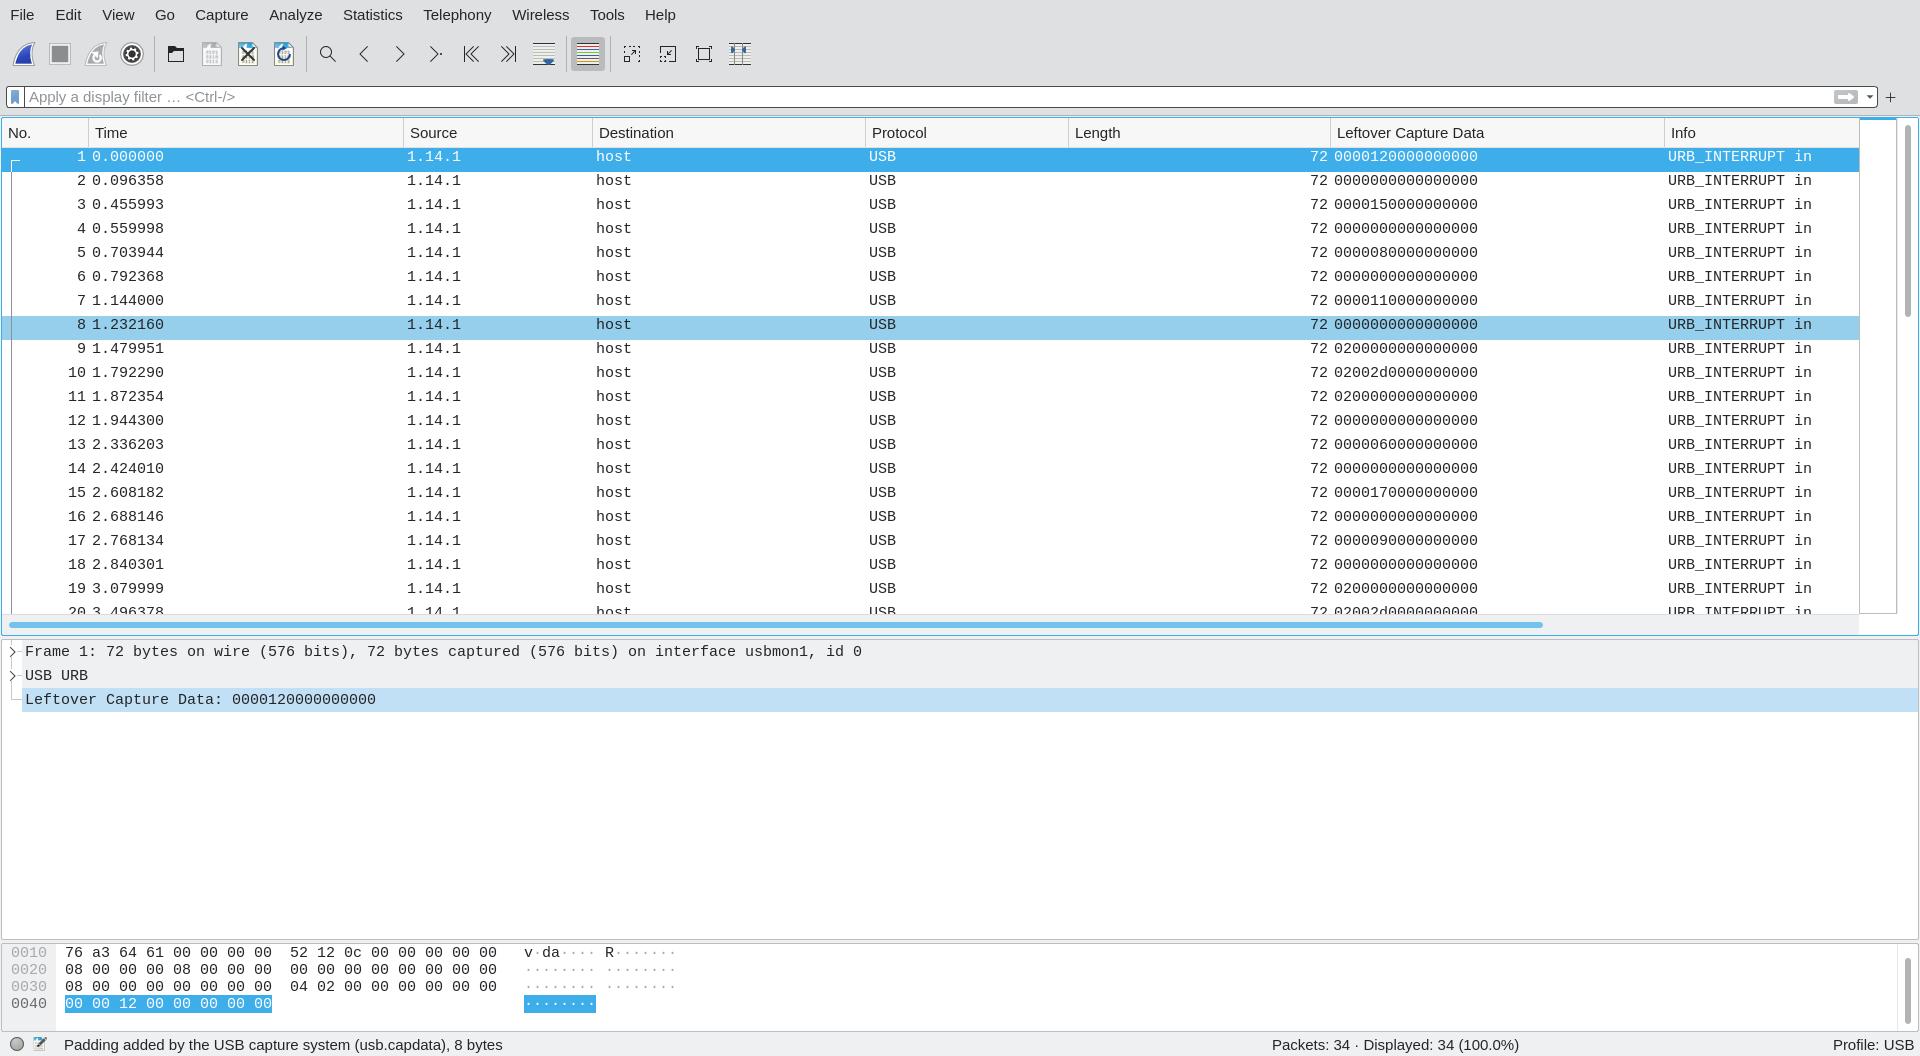
\includegraphics[width=1.0\linewidth]{files/keyboard-payload}
\end{center}
\label{fig:keyboard-payload}
\end{figure}

Экспортируем данные в CSV и убираем заусенцы:
\begin{figure}[H]
\begin{center}
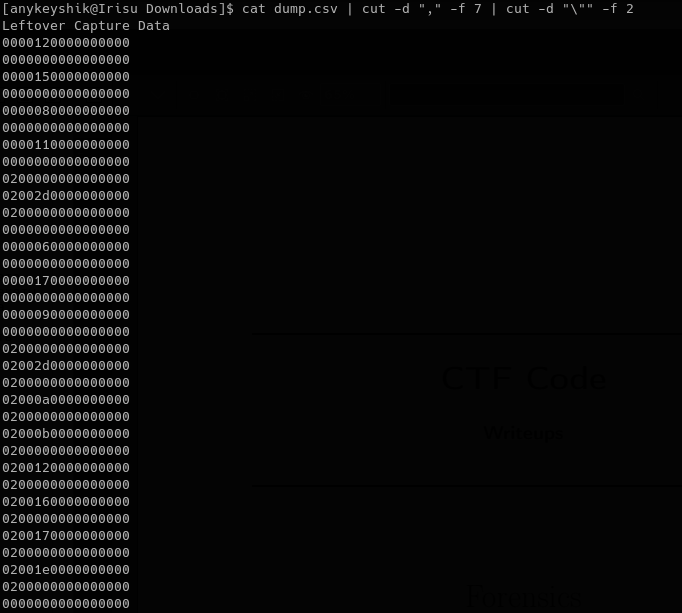
\includegraphics[width=1.0\linewidth]{files/keyboard-csv}
\end{center}
\label{fig:keyboard-csv}
\end{figure}

После чего не составляет проблемы написать простенький питоновский скрипт для парса этой штуки и получения флага:
\begin{lstlisting}[language=Python]
#!/usr/bin/env python3
# -*- coding: utf-8 -*-

keyboardMap = {
    2: "PostFail",
    4: "a",
    5: "b",
    6: "c",
    7: "d",
    8: "e",
    9: "f",
    10: "g",
    11: "h",
    12: "i",
    13: "j",
    14: "k",
    15: "l",
    16: "m",
    17: "n",
    18: "o",
    19: "p",
    20: "q",
    21: "r",
    22: "s",
    23: "t",
    24: "u",
    25: "v",
    26: "w",
    27: "x",
    28: "y",
    29: "z",
    30: "1",
    31: "2",
    32: "3",
    33: "4",
    34: "5",
    35: "6",
    36: "7",
    37: "8",
    38: "9",
    39: "0",
    40: "Enter",
    44: "Space",
    45: "-",
    47: "[",
    48: "]",
    57: "CapsLock"
}

with open('hexoutput', 'r') as keys:
    for line in keys:
        bytesArray = bytearray.fromhex(line.strip())

        for byte in bytesArray:
            if byte != 0:
                value = int(byte)

                if value in keyboardMap:
                    print(keyboardMap[value])
                else:
                    print("Unknown key {:d}!".format(value))
\end{lstlisting}

%-----------------------------------------

\experiment{easy2}

\textbf{Теги:} Виртуальная машина, сброс пароля, дамп памяти\vspace{\baselineskip}

\begin{tcolorbox}
<условие задачи>
\end{tcolorbox}

Нам дается запароленная виртуалка с Windows 7. Хакер, который ее использовал был явно не самым аккуратным человеком, это видно, стоит только зайти. Ну кто будет хранить флаги на рабчоем столе? По сути, вся задача сводится к гуглингу "как сбросить пароль на Windows 7" или, более умный путь решения, знания из которого пригодятся в последней задачи ветки - вытащить из данного дампа памяти с помощью Volatility и плагина mimikatz.

\begin{verbatim}
$ volatility --plugins=%plugin_folder% -f dump.vmem --profile=Win7SP1x64 mimikatz

Volatility Foundation Volatility Framework 2.6.1
Module   User             Domain           Password
-------- ---------------- ---------------- ----------------------------------------
wdigest  Kirino           OreImo           KirinoAyaseBestLove
\end{verbatim}

Подробнее про Volatility можно почитать \href{https://habr.com/ru/post/433248/}{вот здесь}.

Флаг: \verb|oren_ctf_Shellshock!|

%----------------------------------------------------------------------------------------

\labday{Medium}

\experiment{medium1}

\textbf{Теги:} FAT32, циклическая система, дамп\vspace{\baselineskip}

\begin{tcolorbox}
<условие задачи>
\end{tcolorbox}

Нам дан FAT32 дамп какого-то диска. Если немного побродить по папкам становится понятно, что система закольцована. Но должно же быть решение! Если проанализировать дамп \verb|fatcat|'ом (или чем-то похожим), то можно увидеть, что количество ссылок на \verb|O| немного отличается. Стоп, но и флаги наичнаются с \verb|O|. Провалившись вниз еще на несколько уровней становится понятно, что это флаг, зашитый в закольцованный дамп. Дальше можно или ручками пройти весь путь или написать простенький баш-скрипт, который найдет нужный путь:
\begin{lstlisting}[language=Bash]
#!/bin/sh

for i in {1..660}
do
    fatcat dump -L $i 2>/dev/null | grep '^f' >> files
done
\end{lstlisting}

Содержимое файлика весьма лаконично:
\begin{lstlisting}
f 1/1/1980 00:00:00  MATCH                          c=74 s=0 (0B)
f 1/1/1980 00:00:00  MATCH                          c=74 s=0 (0B)
f 1/1/1980 00:00:00  MATCH                          c=74 s=0 (0B)
f 1/1/1980 00:00:00  MATCH                          c=74 s=0 (0B)
\end{lstlisting}

Воспользуемся прямым путем до флага: \verb|fatcat -k 74 dump| и получим \newline \verb|/SPACE/O/R/E/N/_/C/T/F/_/V/E/N/O/M/!/MATCH|. Немного побрутив регистр одного слова (все остальные фиксированы) получем наш флаг: \verb|oren_ctf_VENOM!|.
\newpage

%-----------------------------------------

\experiment{medium2}

\textbf{Теги:} Фазовое кодирование, стеганография\vspace{\baselineskip}

\begin{tcolorbox}
<условие задачи>
\end{tcolorbox}

В аудиозаписи автоматический голос сообщает: "где-то в этом сообщении спрятан флаг". Никакой другой полезной информации голос не сообщает.

Слушаем файл и слышим характерные "потрескивания" на фоне голоса. Эти же потрескивания видны и в спектрограмме (вертикальные линии):
\begin{figure}[H]
\begin{center}
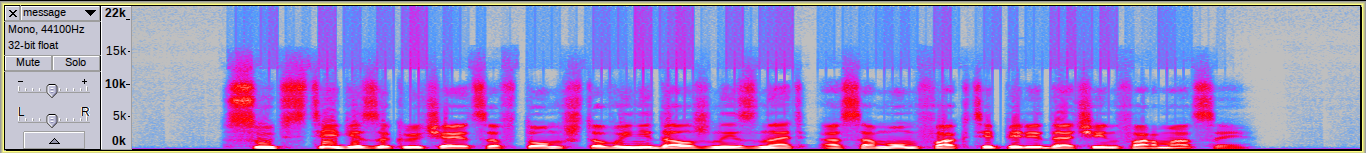
\includegraphics[width=1.0\linewidth]{files/spectrogram}
\end{center}
\label{fig:spectrogram}
\end{figure}

Для тех, кто знаком со звуковой стеганографией, эти потрескивания сразу же напомнят фазовое кодирование — один из самых простых и эффективных методов скрытия информации. Этот метод довольно популярен, и его часто описывают в исследованиях.

Чтобы решить таск, нужно написать (или найти в интернете) код, который умеет разворачивать фазовое кодирование, и перебрать длину сегмента. По простому запросу \href{https://github.com/Galarius/py-stego-phase}{такой} код на Python находится на 4 строке выдачи. Кстати, как раз с помощью этого репозитория и был спрятан флаг!

Если взять тот код, его придётся немного подправить для конкретного WAV файла — он умеет работать только со звуком определённого формата.

Прогоняем обратно, получаем флаг: \verb|oren_ctf_Heartbleed!|

%----------------------------------------------------------------------------------------

\labday{Hard}

\experiment{hard}

\textbf{Теги:} Break random\vspace{\baselineskip}

\begin{tcolorbox}
<условие задачи>
\end{tcolorbox}

Нам дается архив с текстом программы и зашифрованным флагом. Казалось бы, на первый взгляд задача нерешаемая. Но если немного подумать, то становится понятно, что зип-архив дан чтобы восстановить время в которое был проведен xor. Тогда очень просто написать декриптор и получить флаг:
\begin{lstlisting}[language=C++,
					directivestyle={\color{black}}
					emph={int,char,double,float,unsigned},
					emphstyle={\color{blue}}
					]
#include <iostream>
#include <fstream>
#include <ctime>
#include <cstdlib>

int main()
{
    std::fstream in("flag.enc", std::fstream::in);
    std::fstream out("out", std::fstream::out);

 	std::string flag;
 	std::string wtf;
 	time_t start_time;

    in >> flag;
    std::cin >> start_time;

 	while(start_time > 0)
 	{
  		srand(start_time);
  		for(int i = 0; i < flag.size(); i++)
 	 	{
            char ch = flag[i] ^ rand() % 255;
            if (!isprint(ch)) {
                break;
            }
    		
            wtf.push_back(ch);
  		} 
  	
        wtf.push_back('\n');
		out << wtf;
  		start_time -= 1;
 	} 
}	
\end{lstlisting}
				   
Грепаем выходной файлик и получаем флаг \verb|oren_ctf_goto_fail!|

%----------------------------------------------------------------------------------------

\labday{Real life}

\experiment{reallife}

\textbf{Теги:} Анализ памяти\vspace{\baselineskip}

\begin{tcolorbox}
<условие задачи>
\end{tcolorbox}

Казалось бы, на виртуалке уже все посмотрено. Но как-то удивляет хром с девственно-чистой историей. Надо бы посмотреть, что там было. Благо, нам дан дамп оперативной памяти. Просто залезаем плагином в историю хрома и, внезапно, получаем ссылку на pastebin.com, где лежит последний флаг серии.

\begin{verbatim}
volatility --plugins=%plug_folder% -f dump --profile=Win7SP1x64 chromehistory
\end{verbatim}

Флаг: \verb|oren_ctf_Badlock!|

%----------------------------------------------------------------------------------------

\end{document}